\documentclass[fleqn]{article}
\oddsidemargin 0.0in
\textwidth 6.0in
\thispagestyle{empty}
\usepackage{import}
\usepackage{amsmath}
\usepackage{graphicx}
\usepackage{flexisym}
\usepackage{calligra}
\usepackage{amssymb}
\usepackage{bigints} 
\usepackage[english]{babel}
\usepackage[utf8x]{inputenc}
\usepackage{float}
\usepackage[colorinlistoftodos]{todonotes}


\DeclareMathAlphabet{\mathcalligra}{T1}{calligra}{m}{n}
\DeclareFontShape{T1}{calligra}{m}{n}{<->s*[2.2]callig15}{}
\newcommand{\scriptr}{\mathcalligra{r}\,}
\newcommand{\boldscriptr}{\pmb{\mathcalligra{r}}\,}

\definecolor{hwColor}{HTML}{AD53BA}

\begin{document}

  \begin{titlepage}

    \newcommand{\HRule}{\rule{\linewidth}{0.5mm}}

    \center

    \begin{center}
      
\includegraphics[height=11cm, width=11cm]{asu.png}
    \end{center}

    \vline

    \textsc{\LARGE Classical Parts/Field/Matter III}\\[1.5cm]

    \HRule \\[0.5cm]
    { \huge \bfseries Homework 10}\\[0.4cm] 
    \HRule \\[1.0cm]

    \textbf{Behnam Amiri}

    \bigbreak

    \textbf{Prof: Samuel Teitelbaum}

    \bigbreak

    \textbf{{\large \today}\\[2cm]}

    \vfill

  \end{titlepage}

  \begin{enumerate}
    \item \textbf{11.15 (40 points)} Find the angle $\theta_{max}$ at which the maximum radiation is emitted, in
    Ex. 11.3 (Fig. $11.13$). Show that for ultrarelativistic speeds (v close to c), $\theta_{max} \approxeq \sqrt{(1-\beta)/2}$. 
    What is the intensity of the radiation in this maximal direction (in the ultrarelativistic case), in proportion 
    to the same quantity for a particle instantaneously at rest? Give your answer in terms of $\gamma$.
    \emph{Note that this is for on-axis radiation (i.e. Bremstrahlung) which is a bit different from the example we 
    did in class.  Start with Eq. 11.74 in Griffiths, and proceed as we did in class to calculate the emitted intensity.}

      % \textcolor{hwColor}{
      %   \\
      % }

    \item \textbf{12.9 (20 points)} A Lincoln Continental is twice as long as a $VW$ Beetle, when they
    are at rest. As the Continental overtakes the $VW$, going through a speed trap, a
    (stationary) policeman observes that they both have the same length. The $VW$ is
    going at half the speed of light. How fast is the Lincoln going? (Leave your answer
    as a multiple of $c$.)

      % \textcolor{hwColor}{
      %   \\
      % }

    \item \textbf{12.10 (20 points)} A sailboat is manufactured so that the mast leans at an angle $\bar{\theta}$ with
    respect to the deck. An observer standing on a dock sees the boat go by at speed $v$
    (Fig. $12.14$). What angle does this observer say the mast makes?
    \emph{Note that length contraction can help us understand why synchrotron radiation comes out in the 
    forward direction when going from the particle's frame to the observer frame.}
    \begin{center}
      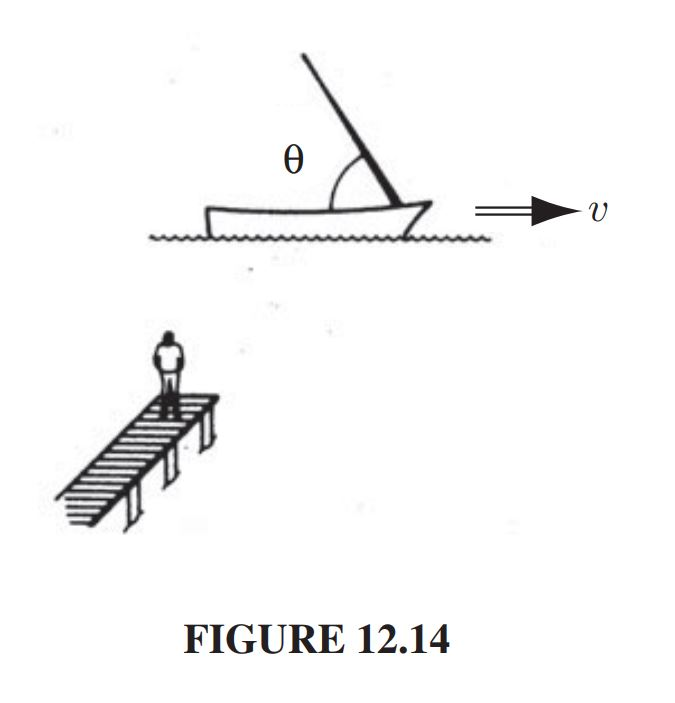
\includegraphics[height=11cm, width=11cm]{1214.JPG}
    \end{center}

      % \textcolor{hwColor}{
      %   \\
      % }

  \end{enumerate}

\end{document}
